% https://github.com/xinychen/awesome-latex-drawing
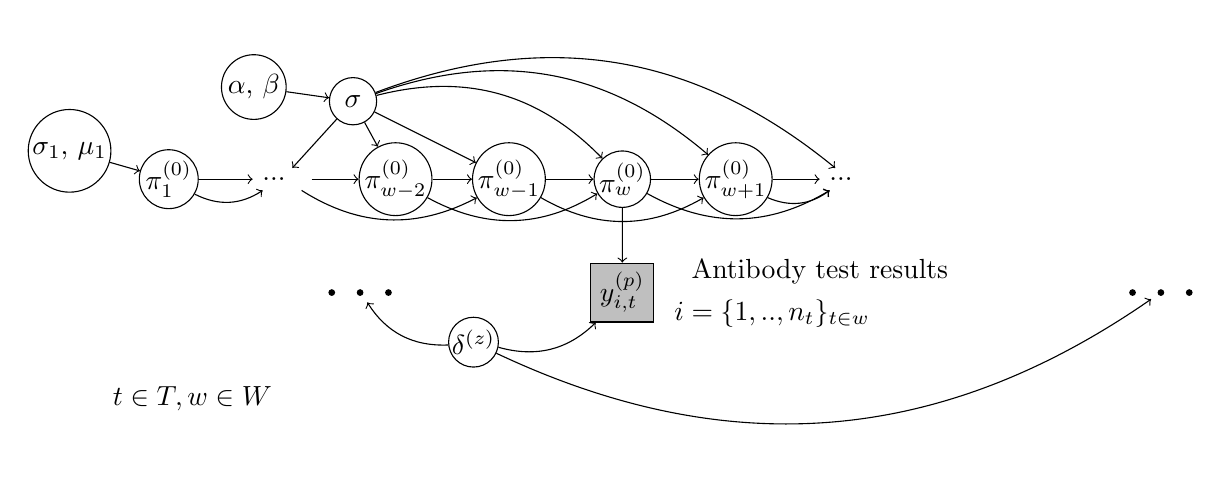
\begin{tikzpicture}[scale=0.9]
    
    % antibody prevalence

    % prior for w 0
    \node [circle,draw=black,fill=white,inner sep=0pt,minimum size=0.6cm] (serow1) at (-1.6,1.6) {$\pi^{(0)}_{1}$};
    
    % ...
    \node [text width=0.5cm] (serodot1) at (0,1.6) {...};  
    
    % w - 2
    \node [circle,draw=black,fill=white,inner sep=0pt,minimum size=0.6cm] (serow-2) at (1.6, 1.6) {$\pi^{(0)}_{w-2}$};
    
    % w - 1
    \node [circle,draw=black,fill=white,inner sep=0pt,minimum size=0.6cm] (serow-1) at (2*1.6, 1.6) {$\pi^{(0)}_{w-1}$};   
    
    % w
    \node [circle,draw=black,fill=white,inner sep=0pt,minimum size=0.6cm] (serow) at (3*1.6, 1.6) {$\pi^{(0)}_{w}$};
    
    % w + 1 ...
    \node [circle,draw=black,fill=white,inner sep=0pt,minimum size=0.6cm] (serow+1) at (4*1.6, 1.6) {$\pi^{(0)}_{w+1}$};
    \node [text width=0.5cm] (serodot2) at (5*1.6,1.6) {...};  
    
    
    % mu 1, sigma 1
    \node [circle,draw=black,fill=white,inner sep=1pt,minimum size=0.6cm] (sigma1) at (-3, 2) {$\sigma_1$, $\mu_1$};
    
    % sigma    
    \node [circle,draw=black,fill=white,inner sep=0pt,minimum size=0.6cm] (sigma) at (1, 2.7) {$\sigma$};
    
    % alpha and beta for sigma
    \node [circle,draw=black,fill=white,inner sep=1pt,minimum size=0.7cm] (ab) at (-0.4, 2.9) {$\alpha$, $\beta$};
   
    \path [draw,->] (ab) edge (sigma); 

    
    % dependencies s -> s direct
     \path [draw,->] (serow1) edge (serodot1);   
     \path [draw,->] (serodot1) edge (serow-2);   
     \path [draw,->] (serow-2) edge (serow-1);   
     \path [draw,->] (serow-1) edge (serow);   
     \path [draw,->] (serow) edge (serow+1);   
     \path [draw,->] (serow+1) edge (serodot2);   
     
    % dependencies s -> s indirect
     \path [draw,->] (serow1) edge [bend right] (serodot1);   
     \path [draw,->] (serodot1) edge [bend right] (serow-1);   
     \path [draw,->] (serow-2) edge [bend right] (serow);   
     \path [draw,->] (serow-1) edge [bend right] (serow+1);   
     \path [draw,->] (serow) edge [bend right] (serodot2);  
     \path [draw,->] (serow+1) edge [bend right] (serodot2);   

 
    % paths for sigma
    \path [draw,->] (sigma) edge (serodot1); 
   \path [draw,->] (sigma1) edge (serow1);   
   \path [draw,->] (sigma) edge (serow-2);   
   \path [draw,->] (sigma) edge (serow-1);   
   \path [draw,->] (sigma) edge [bend left] (serow);   
   \path [draw,->] (sigma) edge [bend left] (serow+1);   
   \path [draw,->] (sigma) edge [bend left] (serodot2); 
  
    
    % Antibody test results
    \node [text width=4cm] (obslabel) at (5*1.6,0.3)  {Antibody test results};  
    
    \node [rectangle,draw=black,fill=lightgray] (yw) at (3*1.6,0) {$y^{(p)}_{i, t}$};  
    
    \node [text width=3cm] (nsero) at (4.5*1.6,-0.3)  {$i = \{1, .., n_{t} \}_{t \in w}$}; 
    
    \plate[] {YW}{(yw)(nsero)(obslabel)}{}

    % dots for obs, left of y
    \node[mark size=1pt,color=black] (ydot1) at (0.7,0) {\pgfuseplotmark{*}};
    \node[mark size=1pt,color=black] (serodotleft) at (0.7+0.4,0) {\pgfuseplotmark{*}};
    \node[mark size=1pt,color=black] at (0.7+0.8,0) {\pgfuseplotmark{*}};
    
    % dots for obs, right of y
    \node[mark size=1pt,color=black] at (7.5*1.6,0) {\pgfuseplotmark{*}};
    \node[mark size=1pt,color=black] (serodotright) at (7.5*1.6+0.4,0) {\pgfuseplotmark{*}};
    \node[mark size=1pt,color=black] (ydot2) at (7.5*1.6+0.8,0) {\pgfuseplotmark{*}};
    
    
    % test specificity
    \node [circle,draw=black,fill=white,inner sep=0pt,minimum size=0.6cm] (spec) at (2.7,-0.7) {$\delta^{(z)}$};

    
   \path [draw,->] (serow) edge (yw);   
   \path [draw,->] (spec) edge [bend right] (yw);   
   \path [draw,->] (spec) edge [bend left] (serodotleft);   
   \path [draw,->] (spec) edge [bend right] (serodotright); 
   

    % study period
    \node [text width=2.5cm] (t) at (-1,-1.5) {$t \in T, w \in W$}; 
    
    % plate for all
    \plate[]{T}{(YW)(spec)(sigma1)(ab)(ydot1)(ydot2)(t)}{}

 
    
\end{tikzpicture}
